\section*{Política Fiscal}
Política fiscal se refere, principalmente, em relação a receitas (arrecadação) e gastos do governo. A receita do governo se da principalmente por meio de tributos, que podem ser divididos em dois grupos: 
\begin{itemize}
    \item Diretos: Sob renda e propriedade (Imposto de Renda, IPVA)
    \item Indiretos: Sob consumo e produção (ICMS,IPI)
\end{itemize}
No Brasil, os tributos arrecadados são indiretos, recaindo "igualmente" entre ricos e pobres.
Já os gastos podem ser descritos como: 
\begin{itemize}
    \item De Capital: Investimento do Governo 
    \item Correntes: Existem 3 subtipos: Consumo,transferência e financeiro. 
\end{itemize}
O Consumo se refere principalmente à manutenção da máquina pública e salários. Já as transferências se referem a benefícios sociais e aposentadorias e por fim, o financeiro se refere a juros da dívida pública. 
Os gastos correntes são frequentemente criticados pois não aumentam o crescimento no Longo-Prazo. 
\subsection*{Curva de Lafer}
A curva de Lafer, basicamente, expoê que existe um limite para a arrecadação de impostos. Como pode ser visto na figura abaixo: 
\begin{figure}[h!]
    \centering
    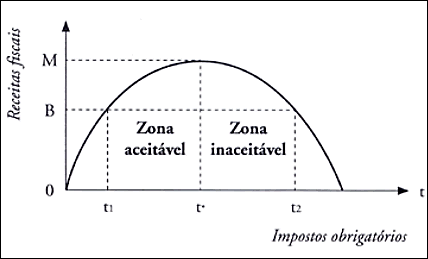
\includegraphics{Elementos do Texto/Figuras/84c4cf1024e60fe5773b5d4ef2615d8b.png}
    \caption{Curva de Laffer padrão}
    \label{Lafer}
\end{figure}
Por essa curva podemos perceber que caso ocorra um aumento muito grande de impostos, pode haver uma evasão fiscal, levando a uma maior informalidade.
\begin{itemize}
    \item Efeito Renda: O imposto aumentando e a pessoa fica mais pobre, trabalhando mais para compensar e a arrecadação aumenta. 
    \item Efeito Substituição: Quanto maior a alíquota de imposto, uma hora trabalhada a mais gera uma renda que não vale a pena trabalhar para. 
\end{itemize}
Na parte crescente, temos um domínio do efeito renda sob o efeito substituição, o contrário ocorre na parte decrescente. 
\subsection*{Indicadores Fiscais}
\begin{itemize}
    \item Indicadores de Fluxo: Défict/Superávit Orçamentário, arrecadação vs gastos em um período. 
    \item Indicadores de Estoque: Dívida 
    \begin{equation}
        D_{t} = (1+i)D_{t-1} - T_{t} + G_{t}
    \end{equation}
    Somatório de déficts acumulado de fluxos do passado
    \item Resultado Primário:
    \begin{equation}
        RP = T_{t} - G_{t}
    \end{equation}
    Estatística de fluxo para um ano, no período $t$
    Receitas ($T$) - Gastos($G$), excluindo receitas e gastos financeiros 
    \item Resultado Nominal, é o Resultado Primário incluindo gastos e receitas financeiras
    \begin{equation}
        RN = (T_{t} - G_{t}) - iD_{t-1}
    \end{equation}
\end{itemize}

A dívida depende de 3 aspectos fundamentais:
\begin{itemize}
    \item Taxa de juros média que inside nela 
    \item Estoque de dívidas já existentes no passado
    \item Resultado Primário 
\end{itemize}
Diminuição de Parte da Dívida é atrelada ao câmbio, melhora de perfil em pré-fixação mostram melhoras na dívida mas ainda é muito grande. Também há de ser ressaltado que a relação dívida-PIB pode dar uma falsa impressão de como o país esta, negligenciando o prazo de pagamento e custo médio da dívida. 
Já o Risco País é o número de pontos percentuais de juros que o país deve pagar em relação a taxa de juros americana (FED) para ser compensado do risco de investir naquele país. 
\subsection*{Regras Fiscais}
Podemos definir Regras Fiscais como um mecanismo que introduz, por um certo período de tempo, limites quantitavios para alguma das principais variáveis fiscais de um país, de acordo com \cite{Giambiagi}, de forma a conter o viés deficitário do setor público. 
A razão para a existência desse viés deficitário, pode ser também explicada por \cite{Giambiagi}, no seguinte trecho do capítulo "Teto de Gastos: O que aconteceu ?" da seu livro "Tudo sobre o défict público: O Brasil na encruzilhada fiscal": 

\begin{citacao}
"A existência desse viés tem diferentes explicações na literatura. A primeira decorre da informação limitada dos agentes econômicos: como muitos desses não enxergam perfeitamente a restrição orçamentária do governo, tendem a superestimar os benefícios dos gastos correntes e subestimar os custos fiscais a ele associados. Uma segunda explicação associa o viés deficitário com ambientes da acirrada competição política. Nesses casos, a dívida pública pode ser usada estrategicamente pelo governante ara influenciar a escolha de seu sucessor. Outra explicação é relacionada a grupos de pressão. Supondo uma sociedade com diferentes grupos que se beneficiam de determinados tipos de gasto, o governo pode ser influenciado pelo lobby desses grupos, levando a um nível orçamentário maior que o desejado." \cite{Giambiagi}
\end{citacao}

Após essa breve exposição, já podemos falar que política fiscal importa e muito, dado que ela diminui a inflação e a fuga de capitais, trazendo estabilidade e credibilidade (transparência), diminuindo o viés inflacionário e levando racionalidade ao orçamento. 
Ter dívida não significa algo ruim, ela pode fazer possíveis escolhas intertemporais ótimas, permite atender a situações emergenciais, permite a estabilização automática, pois é contracíclica e diminui o ciclo, pode agir como um controlador da alíquota de imposto. O grande problema é ter uma dívida muito grande a ponto que o Estado não consiga arcar com ela, o crescimento estável da dívida é bom, o ruim é o crescimento instável e sem controle. 
\subsection*{Teto de Gastos}
Regra Fiscal adotada no final de 2016, válida por até 20 anos e se aplica a 3 esferas distintas do Governo Federal, sendo assim limites individualizados para cada órgão. 
Existem exceções para o Teto, gastos eleitorais não entram nele, investimentos em gastos de capital também não entram. 
\subsection*{Equivalência Ricardiana}
A equivalência ricardiana possui como pressuposto básico que o consumidor se importa com o consumo no período corrente (hoje) e no período posterior a ele (amanhã). O consumidor racional, sabe que dado uma queda na arrecadação tributária hoje é equivalente a mais impostos no futuro.Trazendo isso para uma interpretação mais macro, isso indica que o aumento das despesas do Governo ou corte nos impostos não gera aumento da demanda agregada no curto-prazo. 
Essa visão possui duas principais críticas, uma relacionada a racionalidade dos agentes, dado que eles podem não ser 100$\%$ racionais a todo tempo, podendo ser miopes e também a critica de Keynes acerca disso: "um aumento dos gastos governamentais pode sim aumentar o nivel de demanda agregada por causa do efeito multiplicador."